\documentclass[entwurf.tex]{subfiles}

\begin{document}
\chapter{Klassendiagramme}
	\section{Bus}
		
  		In diesem Diagramm ist der Aufbau des Moduls ''Bus'' zu sehen. Die Kommunikation zwischen allen Modulen ist entkoppelt und findet größtenteils über den Austausch von Nachrichten verschiedener Typen über den Bus statt. Um mit dem Bus arbeiten zu können, muss ein Modul eine Klasse besitzen, die von der abstrakten Klasse ''BusDevice'' erbt. Der Bus funktioniert als eine Variation des Beobachter-Entwurfsmusters. Eine von ''BusDevice'' erbende Klasse kann über subscribe() bzw. unsubscribe() auf dem ''MessageBus'' Nachrichten eines bestimmten Themas (``Topic'') (Sensortyp, Datenbanknachrichten, Konfigurationsnachrichten, ...) abonnieren und Abonnements beenden. \\
  		Diese Abonnements werden in der Klasse ''Broker'' verwaltet. Sendet eine Instanz von ''BusDevice'' über publish() eine Nachricht an ''MessageBus'', so holt sich letzterer von seinem Broker eine Liste über alle Abonnements für das Topic der Nachricht und sendet diese dann an alle abonnierenden Objekte. Das versenden einer Nachricht sowie deren Empfang sind asynchrone Funktionsaufrufe. \\
  		Die abstrakte Klasse ''Message'' besitzt eine Reihe von erbenden Klassen. Dies ist nötig, um alle möglichen Typen von Nachrichten darzustellen: ''SensorValueMessage'' wird für das einfache versenden von Messwerten benutzt, ''ConfigFileRequest'' für Konfigurationsdateien usw. Dieser Aufbau ermöglicht das leichte Ergänzen um ggf. zusätzlich benötigte Nachrichtentypen. Ein besonderer Nachrichtentyp ist die 'DatabaseRequestMessage', die Anfragen an die Datenbank beinhaltet. Die Anfragen vom Typ ''DBRequest'' sind unterteilt in verschiedene Typen von Anfragen: DBReqRecent fordert die letzten n Einträge an, DBReqFrom alle Einträge seit einem bestimmten Datum, und DBReqRange fordert alle Datenbankeinträge zwischen zwei Daten an. \\
  		Das Konstrukt der Klassen ''BusDevice'' sowie erbende Klassen, ''Message'' und die von ''Message'' erbenden Klassen ergeben gemeinsam das Entwurfsmuster der Fabrikmethode.
  		
  		\begin{figure}[H]
  			\begin{center}
 				\makebox[\textwidth][c]{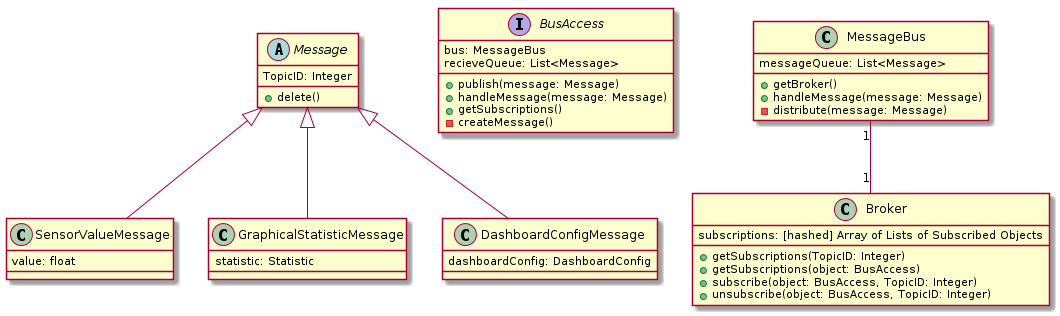
\includegraphics[width=0.8\paperheight, angle=90]{diagrams/Bus.png}}
  				\caption{Bus Klassendiagramm}
  			\end{center}
  		\end{figure}
  	
  	\newpage
  	\section{Virtuelle Sensoren}
		Virtuelle Sensoren berechnen aggregierte Funktionen aus Sensorwerten. Die Klasse ''VirtualSensor'' ist ein BusDevice. Es gibt (grundlegend unterschiedliche) Arten von Virtuellen Sensoren. Der momentane Benzinverbrauch ist ein Live-Datum, welches aus mehreren Live-Sensordaten berechnet wird. Die generierten Daten sind insbesondere unabhängig vom Zustand der Datenbank. Ein virtueller Sensor, der einen Durchschnittswert über eine bestimmte Zeit berechnet, benötigt Daten aus der Datenbank. Die Anfrage wird über den Bus geschickt (~\ref{vsseq}). Der virtuelle Sensortyp ''TopicOverTime'' schickt nach einem Datenbankrequest nacheinander Messages mit Tupeln aus Zeit und Wert auf den Bus. Ein solcher Virtueller Sensor (wie Durchschnittswert und ''TopicOverTime'') ist abhängig vom Zustand der Datenbank.

		Die Berechnung einer zustandsabhängigen aggregierten Funktion erfolgt durch eine einmalige Initialisierung des Virtuellen Sensors mit Daten aus der Datenbank. Danach werden die Daten direkt vom virtuellen Sensor inkrementell berechnet.

		Es gibt die virtuellen Sensoren:
		\begin{itemize}
			\item{TopicOverTime:} Die einfachste Art eines zustandsabhängigen virtuellen Sensors. Schickt, wenn requested, Tupel aus Zeit und Wert des spezifierten Topics.
			\item{TripMileage:} Berechnet den Kilometerstand der Fahrt ab einem spezifiziertem Zeitpunkt.
			\item{FuelConsumption:} Berechnet den Momentanverbrauch
			\item{RemainingMiles:} Berechnet die verbleibenden Kilometer. Die Berechnung ist abhängig vom Fahrverhalten des aktuellen Fahrers.
			\item{AverageComputation:} Liefert den Durchschnittswert eines spezifizierten Topics.
		\end{itemize}

		\begin{figure}[H]
  			\begin{center}
 				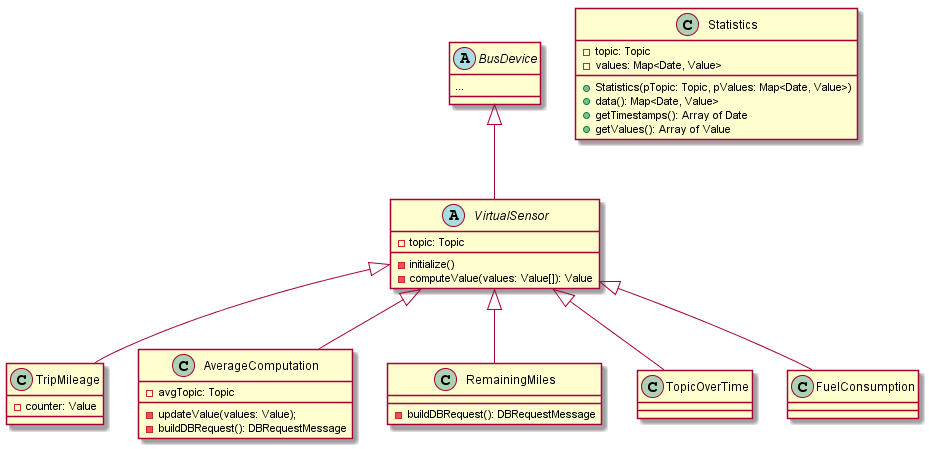
\includegraphics[width=0.8\textheight,angle=90]{diagrams/VirtualSensors.png}
  				\caption{Klassendiagramm der virtuellen Sensoren}
  			\end{center}
  		\end{figure}
  	\newpage
  	\section{Database Access}
  		Im folgenden Diagramm ist der Aufbau der Datenbank und des Datenbankzugriffs zu sehen.
  		\begin{figure}[H]
  			\begin{center}
 				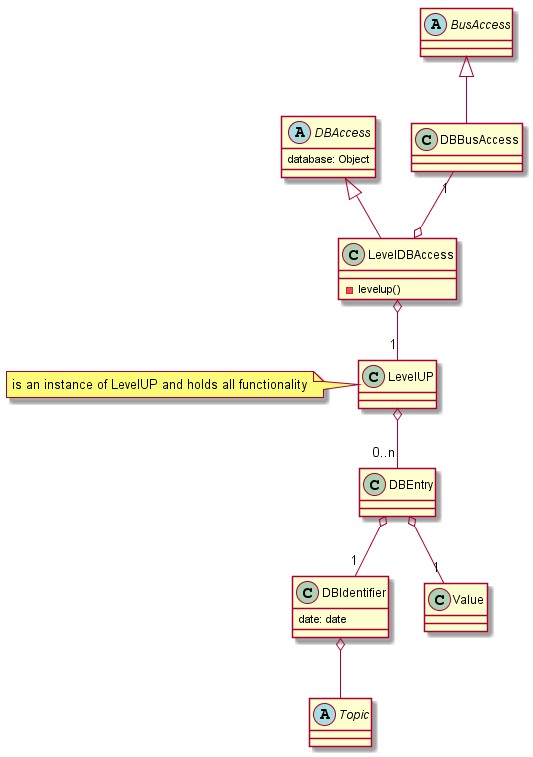
\includegraphics[width=0.8\textwidth]{diagrams/DBAccess.png}
  				\caption{Klassendiagramm des Datenbankzugriffs}
  			\end{center}
  		\end{figure}
  	Als Datenbanksystem wird, wie im Pflichtenheft spezifiziert, LevelDB benutzt. In der LevelDBAccess-Klasse wird außer der Referenz auf die LevelUp-Instanz auch der aktuelle Fahrer sowie die spezifizierte maximale Kapazität der Datenbank gespeichert. \\ In der Datenbank, im Fall von LevelDB ein einfacher Key-Value-Store, werden zwei Typen von Objekten gehalten: Zum einen werden mit der Zeit und dem Typ des Sensors als Key Objekte von Sensorwerten und derzeitigem Fahrer gespeichert. Zum anderen existieren fahrerbezogene Einträge, die den präferierten Kraftstoff des Fahrers sowie die Konfiguration des virtuellen Armaturenbretts beinhalten und mit der Identifikation des Fahrers als Key gespeichert werden. Zur Kommunikation mit anderen Modulen besitzt der Datenbankzugriff mit 'DBBusDevice' eine Klasse, die den Zugang zum Bus möglich macht und Nachrichten vom Bus dekodiert. 
  	
  	\newpage
  	\section{ConfigFileReader \& AvailableSignals}
  		Verschiedene, selten geänderte Informationen werden in einer Konfigurationsdatei gespeichert. Diese Informationen kann der ConfigFileReader ändern. Er reagiert auf bestimmte Requests auf dem Messagebus.
  		
  		Eine weitere wichtige Information ist, welche Datensignale allgemein zur Verfügung stehen. Dies wird im SignalCollector gespeichert. Er reagiert ebenso auf bestimmte Signale auf dem Bus.
  		\begin{figure}[H]
  			\begin{center}
 				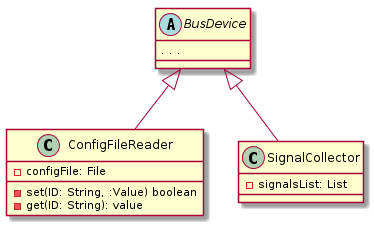
\includegraphics[width=0.8\textwidth]{diagrams/Classes_Config.png}
  				\caption{Klassendiagramm des Config-Readers und SignalsCollector}
  			\end{center}
  		\end{figure}
  	

	\newpage
  	\section{Website}
  	\label{Class:Website}
		Im folgenden Diagramm ist dargestellt, wie die Website allgemein aufgebaut ist. Die Seite besteht aus zwei Frames. In einem Frame wird die Statusleiste angezeigt, im anderen werden können verschiedene Sichten angezeigt werden, darunter unter anderem das GridView, auf welchem die Dashes angezeigt werden. Für weiteres siehe: \nameref{Class:GridView}, \nameref{Class:SettingsView}.
		
		Die Elemente der Statusleiste können unter anderem Text, Knöpfe und Icons sein.
		\begin{figure}[H]
  			\begin{center}
 				\makebox[\textwidth][c]{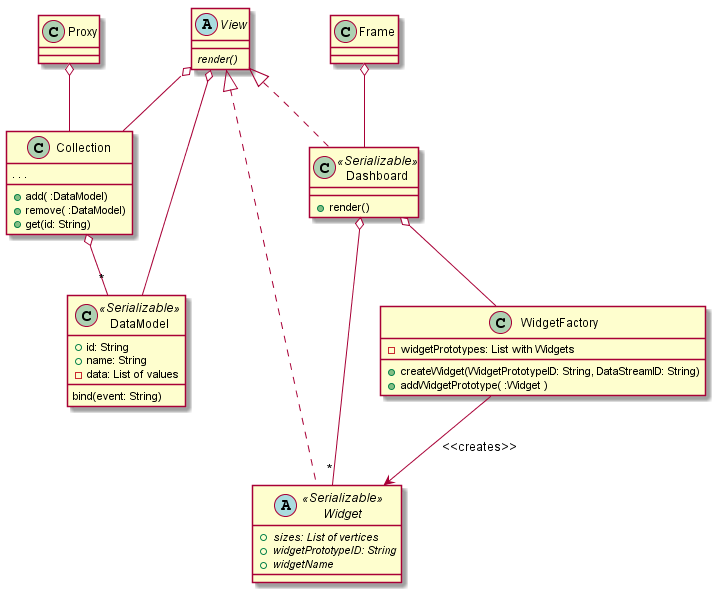
\includegraphics[width=0.8\paperwidth]{diagrams/website.png}}
  				\caption{Klassendiagramm der GUI}
  			\end{center}
  		\end{figure}  	
  	
  	\newpage
  	\section{User Interface}
		Wie in \ref{Class:Website} zu sehen ist, besteht ein Hauptteil des User Interface aus dem ViewFrame, der von verschiedenen Views vertreten werden kann. Im Folgenden sieht man den Aufbau des GridViews und des SettingViews. Das Grid nutzt ein Objekt der Klasse 'Gridster' aus der Bibliothek 'Gridster'. Das GridView besteht hauptsächlich aus diesem Objekt. Es ermöglicht die Anzeige verschiedener Widgets in einem Grid mit Elementen verschiedener Größe.
		
		Hierbei sind die Widgets selbst Abonnenten des angezeigten Signals, weshalb sie die abstrakte Klasse BusDevice implementieren müssen.
		
		Über die SettingsView ist es möglich, verschiedene Widgets in diesem Grid hinzuzufügen oder zu ändern. Aus diesem Grund speichert SettingView immer die Instanz des Grids als Objekt. Dies wird benutzt, wenn z.B. ein früherer Zustand des Grids wiederhergestellt werden soll. Um früher gespeicherte Konfigurationen vom Bus zu empfangen und neue Einstellungen an den Server zu schicken implementiert auch die SettingsView das BusDevice. 
		
		\begin{figure}[H]
  			\begin{center}
 				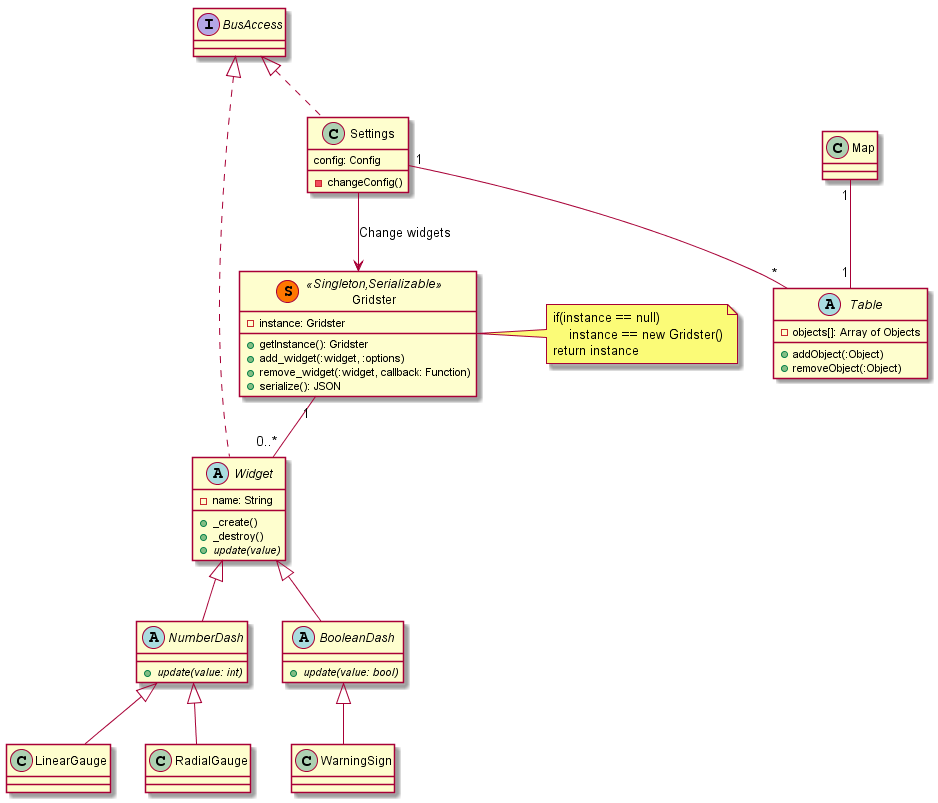
\includegraphics[width=\textwidth]{diagrams/UI.png}
  				\caption{Klassendiagramm der GUI}
  			\end{center}
  		\end{figure}
  	
		\newpage
		\section{Einparkhilfe Ultraschallsensoren}
		Auf dem Server sind keine Berechnungen für die Ultraschallsensoren notwendig. Die neuen Werte werden ständig via WebRTC auf das Endgerät geschickt und dort interpretiert. Auf dem Endgerät werden auch keine Berechnungen durchgeführt, es werden lediglich Messwerte (Distanz) in Farben umgewandelt (ProximityDisplayRefresher).

		\section{Einparhilfe Lenkradposition}
Die Berechnungen der Einparkhilfe werden auf dem Server durchgeführt (Thin-Client-Prinzip). Bei einer Änderung der Lenkradposition wird der Pfad (Path) neu berechnet. Der PathCalculator erzeugt einen neuen Pfad. Die PKW-bezogenen Daten, die in Settings gespeichert sind werden dafür verwendet (carWidth, ... usw.). Falls die Daten nicht vorhanden sind, werden sie von der Datenbank geholt. Danach wird berechnet, wie die Kurve auf dem Bildschirm angezeigt werden soll. Die benötigte Daten sind ebenfalls in Settings gespeichert (camPosition, ... usw.). Danach wird der Pfad auf den Bus gelegt und Richtung Endgerät weitergeleitet. Auf dem Endgerät erfolgen keine Berechnungen. Wenn die Daten (SVG-Path-Koordinaten oder Koordinaten für Bezierkurven) ankommen, wird das SVG-Bild neu gezeichnet (PathRefresher).
  	
		\newpage
  	\section{Einparkhilfe Serverseite}
		Im folgenden Diagramm ist der Aufbau des Rückfahrassistenzsystems auf der Serverseite dargestellt.
		\begin{figure}[H]
 			\makebox[\textwidth][c]{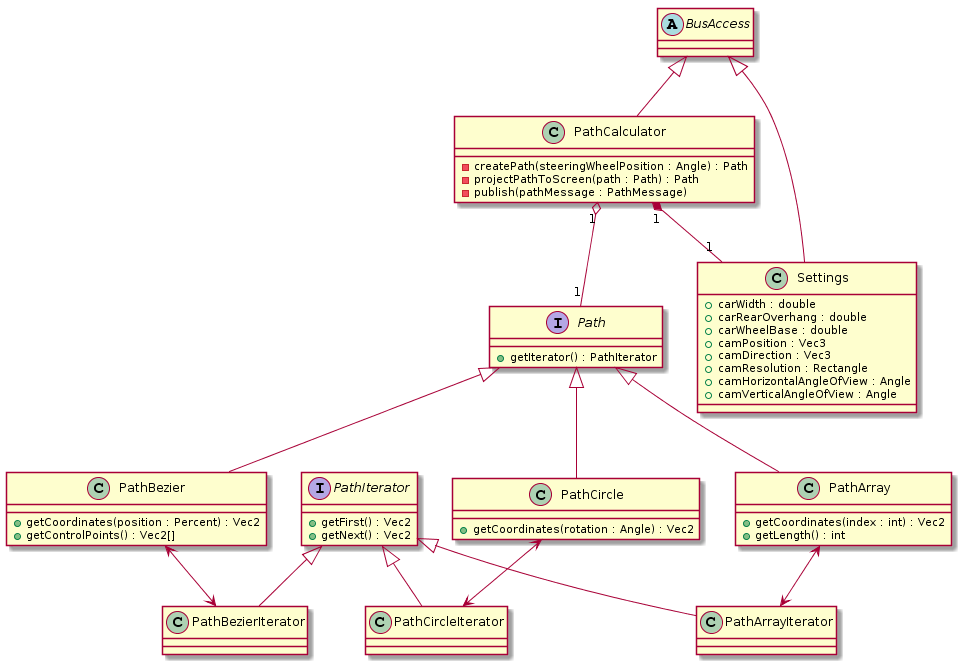
\includegraphics[width=\textwidth]{diagrams/ParkingSensor/v3/classdiagram_server.png}}
  			\caption{Klassendiagramm des Rückfahrassistenzsystems (1)}
  		\end{figure}
  		
  	\newpage
  	\section{Einparkhilfe Clientseite}
		Im folgenden Diagramm ist der Aufbau des Rückfahrassistenzsystems auf der Clientseite dargestellt
		\begin{figure}[H]
 			\makebox[\textwidth][c]{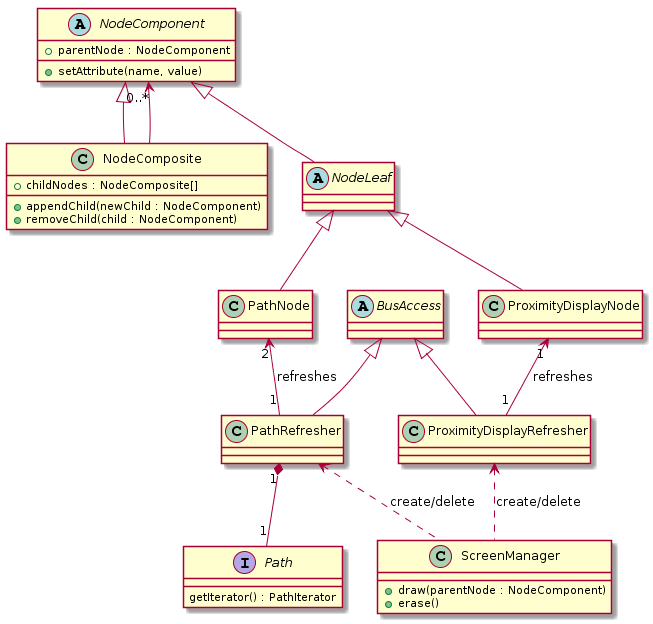
\includegraphics[width=\textwidth]{diagrams/ParkingSensor/v3/classdiagram_userdevice.png}}
  			\caption{Klassendiagramm des Rückfahrassistenzsystems (2)}
  		\end{figure}
  	
  	
\chapter{Klassen}
		\section{Einparkhilfe Clientseite}
	\subsection{NodeComponent}
	\label{Abstract Class:NodeComponent}
		Eine DOM-Komponente, entweder Kompositum oder Blatt (Kompositum-Entwurfsmuster).
		\begin{description}
			\attr{public parentNode: NodeComponent}
				Der Elternknoten dieser NodeComponent.
			\method{public setAttribute(name: var, value: var)}
				Setzt den Wert eines Attributs in NodeComponent.\\
				\textbf{Parameter:} Der Name und der Wert des Attributs.\\
		\end{description}
		
	\subsection{NodeComposite}
	\label{Class:NodeComposite}
		Ein DOM-Kompositum (Kompositum-Entwurfsmuster).
		\begin{description}
			\attr{public childNodes: NodeComposite[]}
				Die Liste aller Kindknoten.
			\method{public appendChild(newChild : NodeComponent)}
				Fügt einen neuen Kindknoten hinzu.\\
			\method{public removeChild(child : NodeComponent)}
				Entfernt einen bereits vorhandenen Kindknoten.\\
		\end{description}
	
	\subsection{NodeLeaf}
	\label{Abstract Class:NodeLeaf}
		Ein DOM-Blatt (Kompositum-Entwurfsmuster).
		
	\subsection{PathNode}
	\label{Class:PathNode}
		Ein DOM-Blatt, das einen Pfad auf dem Bildschirm anzeigt.

	\subsection{PathRefresher}
	\label{Class:PathRefresher}
		Zeichnet die zwei PathNodes neu, wenn die Lenkradposition geändert wird.
		
	\subsection{ProximityDisplayNode}
	\label{Class:ProximityDisplayNode}
		Ein DOM-Blatt, das den Wert eines Ultraschallsensors auf dem Bildschirm visualisiert. Wenn es mehrere Ultraschallsensoren gibt, dann sind mehrere ProximityDisplayNodes notwendig.
		
	\subsection{ProximityDisplayRefresher}
	\label{Class:ProximityDisplayRefresher}
		Aktualisiert das ProximityDisplayNode-Blatt, wenn der Wert des Sensors geändert wird.

	\subsection{ScreenManager}
	\label{Class:ScreenManager}
		Verwaltet die gesamte Darstellung, zeichnet die grafischen Elemente
		\begin{description}
			\method{public draw(parentNode: NodeComponent)}
				Zeichnet alle Anzeigeelemente auf den Bildschirm und initialisiert die Webcam.\\
				\textbf{Parameter:} Der Elternknoten, in dem die Anzeigeelemente gezeichnet werden sollen.
			\method{erase()}
				Löscht alle Anzeigeelemente und stoppt die Videoübertragung.
		\end{description}

	
	\section{Einparkhilfe Serverseite}
	\subsection{Path}
	\label{Interface:Path}
		Das Interface für alle Pfade.
		\begin{description}
			\method{public getIterator() : PathIterator}
				Holt den Iterator, der die aktuelle Implementierung von Path unterstützt.
				\textbf{Rückgabewert:} Ein PathIterator, der die Punkte dieses Pfades durchlaufen kann.
		\end{description}
		
	\subsection{PathIterator}
	\label{Interface:PathIterator}
		Das Interface für den Pfad-Iterator.
		\begin{description}
			\method{public getFirst(): Vec2}
				Holt den ersten Punkt des Pfades.
				\textbf{Rückgabewert:} Die Koordinaten des Punktes.
			\method{public getNext(): Vec2}
				Holt den nächsten Punkt des Pfades.
				\textbf{Rückgabewert:} Die Koordinaten des Punktes.
		\end{description}
	
	\subsection{PathCircle}
	\label{class:PathCircle}
		Eine Path-Implementierung, kann verwendet werden um effizient kreisförmige Pfade zu beschreiben. Damit können die einzelne Punkte des Pfades bei Bedarf einfach berechnet werden.
		\begin{description}
			\method{public getCoordinates(rotation: Angle) : Vec2}
				Holt die Koordinaten eines Punktes, der sich auf dem Kreis befindet. Der Punkt ist wie folgt spezifiziert: es gibt ein Vektor, der vom Mittelpunkt des Kreises zu dem Pfad-Startpunkt zeigt (der Startpunkt ist auf der Kreislinie). Dieser Vektor wird dann gedreht (um "rotation") und der Punkt zu dem der Vektor dann zeigt soll zurückgegeben werden. Der Iterator soll die Funktion mit rotation=0 aufrufen, falls getFirst() aufgerufen wurde. Bei getNext() soll der Winkel jeweils inkrementiert werden.
				\textbf{Parameter:}	Die Drehung des Vektors. Alle möglichen Winkel sind gültig.\\
				\textbf{Rückgabewert:} Die Koordinaten des Punktes auf der Kreislinie.
		\end{description}
	
	\subsection{PathCircleIterator}
	\label{class:PathCircleIterator}
		Ein Iterator, der PathCircle unterstützt.

	\subsection{PathArray}
	\label{class:PathArray}
		Eine Path-Implementierung, kann verwendet werden um allgemeine Pfade einfach speichern zu können. Die Punkte des Pfades werden als Polygonzug gespeichert.
		\begin{description}
			\method{public getCoordinates(index: int) : Vec2}
				Holt den n-ten Punkt des Polygonzuges, falls index = n.
				\textbf{Parameter:} Spezifiziert den Punkt im Polygonzug. Falls der Polygonzug aus m Punkten besteht, dann sind die index-Werte zwischen 0 und m-1 gültig. Falls der index-Parameter ungültig ist, soll null zurückgegeben werden.\\
				\textbf{Rückgabewert:} Die Koordinaten des Punktes.
			\method{public getLength()}
				Holt den Anzahl der Punkte im Polygonzug.
				\textbf{Rückgabewert:} Es wird der Anzahl der Punkte im Polygonzug zurückgegeben.
		\end{description}
		
	\subsection{PathArrayIterator}
	\label{class:PathArrayIterator}
		Ein Iterator, der PathArray unterstützt.

	\subsection{PathBezier}
	\label{class:PathBezier}
		Eine Path-Implementierung, kann verwendet werden um bei der Speicherung von Kurven Platz zu sparen.
		\begin{description}
			\method{public getCoordinates(position: Percent) : Vec2}
				Holt die Koordinaten eines Punktes, der sich auf der Bezierkurve befindet.
				\textbf{Parameter:} Bezier-Parameter t der Kurve [0, 1].
				\textbf{Rückgabewert:} Die Koordinaten des Punktes auf der Bezierkurve.
			\method{public getControlPoints() : Vec2[]}
				Holt die Koordinaten aller Kontrollpunkten der Bezierkurve.
				\textbf{Rückgabewert:} Die Koordinaten aller Punkten auf der Bezierkurve.
		\end{description}
		
	\subsection{PathBezierIterator}
	\label{class:PathBezierIterator}
		Ein Iterator, der PathBezier unterstützt.

	\subsection{Settings}
	\label{class:Settings}
		Hier werden die Kraftfahrzeug- und Kamerabezogenen Parameterwerte bei Bedarf von der Datenbank geholt und gepuffert.
		\begin{description}
			\attr{public carWidth : double}
				Die Breite des Fahrzeugs in Meter.
			\attr{public carRearOverhang : double}
				Der hintere Überhang des Fahrzeugs in Meter.
			\attr{public carWheelBase : double}
				Der Radstand des Fahrzeugs in Meter.
			\attr{public camPosition : Vec3}
				Die Position der Kamera in Fahrzeugkoordinatensystem.
			\attr{public camDirection : Vec3}
				Die Richtung der Kamera in Fahrzeugkoordinatensystem.
			\attr{public camResolution : Rectangle}
				Die Auflösung der Kamera in Pixeln.
			\attr{public camHorizontalAngleOfView : Angle}
				Der horizontale Winkel der Kamera.
			\attr{public camVerticalAngleOfView : Angle}
				Der vertikale Winkel der Kamera.
		\end{description}

	\subsection{PathCalculator}
	\label{class:PathCalculator}
		Hört den Bus ab und erzeugt einen neuen Pfad, und leitet diesen an das Endgerät weiter, falls die Position des Lenkrads geändert wurde.
			\begin{description}
				\method{private createPath(steeringWheelPosition : Angle) : Path}
					Erzeugt einen Pfad der die Bewegung des Fahrzeugs in der Zukunft beschreibt. Der Pfad ist im Fahrzeugkoordinatensystem angegeben. Die zwei gespeicherten Koordinaten sind entlang der x- und z-Achsen, die y-Koordinaten sind 0 für alle Punkte und müssen deswegen nicht gespeichert werden.
					\textbf{Parameter:} Die Position des Lenkrads (Uhrzeigersinn).
					\textbf{Rückgabewert:} Der Pfad, der die Bewegung des Fahrzeugs in der Zukunft beschreibt.
				\method{private projectPathToScreen(path : Path) : Path}
					Projiziert einen Pfad auf den Kamerabildschirm.
					\textbf{Parameter:} Der Pfad der Fahrzeugbewegung in Fahrzeugkoordinatensystem.
					\textbf{Rückgabewert:} Der Pfad der Fahrzeugbewegung in Kamerakoordinatensystem.
				\method{private publish(pathMessage: PathMessage)}
					Sendet eine Nachricht mit dem Pfad an das Endgerät.
					\textbf{Parameter:} Die Nachricht, die den Pfad (in Kamerakoordinatensystem) enthält.
			\end{description}
			
		
	
	\section{Bus}
	\subsection{BusDevice}
	\label{Class:BusDevice} 
		Eine abstrakte Klasse, deren erbende Klassen Zugriff auf das Bus-Modul haben.
		\begin{description}
			\attr{private messages: List of Messages} 
				Noch zu versendende Nachrichten
			\method{public publish(message: Message): Boolean}
			
				Sendet eine Nachricht asynchron an eine Instanz von MessageBus.\\ 
				\textbf{Parameter:} Die zu versendende Nachricht.\\ 
				\textbf{Rückgabewert:} Boolean, der beschreibt, ob die Nachricht beim Bus angekommen ist.
				
			\method{abstract public handleMessage(message: Message): Void}  
				Funktion zum asynchronen Empfangen einer Nachricht von einer Instanz von MessageBus.
				
			\method{public subscribe(object: BusDevice, topic: Topic): boolean} 
				Funktion zum abonnieren von Nachrichten eines bestimmten Themas.\\ 
				\textbf{Parameter:} Der Abonnent und das abonnierte Thema.\\ 
				\textbf{Rückgabewert:} Boolean, der beschreibt, ob das Thema erfolgreich abonniert wurde.
				
			\method{public unsubscribe(object: BusDevice, topic: Topic): boolean} 
				Funktion zum Beenden eines Abonnements zu einem bestimmten Thema.\\ 
				\textbf{Parameter:} Der Abonnent und das abonnierte Thema.\\ 
				\textbf{Rückgabewert:} Boolean, der beschreibt, ob das Thema erfolgreich aus der Liste der Abonnements entfernt wurde.
			\method{private createMessage(): Message} 
				Funktion zum Erzeugen einer neuen Nachricht. Die Funktion sollte in den meisten Fällen von der erbenden Klasse überschrieben werden. \\
				\textbf{Rückgabewert}: Die neu erzeugte Nachricht.
		\end{description}
  		
	\subsection{Message}
	\label{Class:Message} 
		Eine abstrakte Klasse, die als Muster für alle Nachrichten dient, die über den Bus versendet werden können.
		\begin{description}
			\attr{protected topic: Topic}  
				Das Thema der Nachricht; wird zur Identifikation des Nachrichtentyps sowie des Inhalts der Nachricht benutzt.
			\attr{Inhalt}
				Der Inhalt der Nachricht, ist je nach erbender Klasse von einem unterschiedlichen Typ.
		\end{description}
	\subsection{MessageBus}
	\label{Class:MessageBus}
		Die Klasse, die die Funktionalität des Busses beinhaltet.
		\begin{description}
			\attr{private broker: Broker}
				Der Broker des Busses; siehe Beschreibung der Broker-Klasse. 
				
			\method{protected subscribe(object: BusDevice, topic: Topic): Boolean}
			Funktion, die für eine Instanz von BusDevice auf ein Thema eine Subscription in der Broker-Instanz des MessageBus anlegt. \\
			\textbf{Parameter:} Der Abonnent und das abonnierte Thema. \\
			\textbf{Rückgabewert:} Boolean, der den Erfolg des Eintrags der Subscription angibt. 
			
			\method{protected unsubscribe(object: BusDevice, topic: Topic): Boolean}
			Funktion, die für eine Instanz von BusDevice auf ein Thema eine Subscription in der Broker-Instanz des MessageBus löscht, sofern diese existiert. \\
			\textbf{Parameter:} Der Abonnent und das un-abonnierte Thema. \\
			\textbf{Rückgabewert:} Boolean, der angibt, ob keine Subscription (mehr) von dem angegebenen Abonnenten auf das angegebene Thema im Broker eingetragen ist. 
			
			\method{protected handleMessage(message: Message): Void}
			Funktion, die asynchron eine Nachricht von einer Instanz von BusDevice empfängt, sich von der lokalen Broker-Instanz alle Subscriptions auf das Thema der Nachricht holt, und die Nachricht dann über einen Aufruf von distribute(message: Message, subscribers: List of BusDevice) an Instanzen von BusDevice verteilt. \\
			\textbf{Parameter:} Die versendete Nachricht.
			
			\method{private distribute(message: Message, subscribers: List of BusDevice): Void}
			Funktion, die eine Nachricht an alle angegebenen Instanzen von BusDevice versendet.
			\textbf{Parameter:} Die zu versendende Nachricht und eine Liste aller Instanzen von BusDevice, die die Nachricht bekommen sollen. 
			\end{description}
			
		\subsection{Broker}
		\label{Class:Broker}
		Die Klasse, die im Bus alle Abonnements hält und auf Bedarf an den MessageBus zurückgibt.\\
		
		\begin{description}
		\method{getSubscribers(topic: Topic): List of Subscriptions}
		Funktion, die die Liste aller Abonnenten auf ein bestimmtes Thema zurückgibt. \\
		\textbf{Parameter:} Das Thema, auf welchem alle Abonnenten zurückgegeben werden sollen.	\\
		\textbf{Rückgabewert:} Eine Liste aller Abonnenten auf das Thema.	
		

		\method{getSubscriptions(object: BusDevice): List of Topics}
		Funktion, die die Liste aller Abonnements einer bestimmten Instanz von BusDevice zurückgibt. \\
		\textbf{Parameter:} Die Instanz von BusDevice, für die alle Abonnements zurückgegeben werden sollen.	\\
		\textbf{Rückgabewert:} Eine Liste aller Themen, für die die Instanz von BusDevice Abonnements hält. 	
		
		\method{public subscribe(object: BusDevice, topic: Topic): Boolean}
		Funktion, die für eine Instanz von BusDevice auf ein Thema eine Subscription anlegt. \\
		\textbf{Parameter:} Der Abonnent und das abonnierte Thema. \\
		\textbf{Rückgabewert:}Boolean, der den Erfolg des Eintrags der Subscription angibt. 
		
		\method{public unsubscribe(object: BusDevice, topic: Topic): Boolean}
		Funktion, die für eine Instanz von BusDevice auf ein Thema eine Subscription löscht, sofern diese existiert. \\
		\textbf{Parameter:} Der Abonnent und das un-abonnierte Thema. \\
		\textbf{Rückgabewert:} Boolean, der angibt, ob keine Subscription (mehr) von dem angegebenen Abonnenten auf das angegebene Thema eingetragen ist. 
		\end{description}
		
		\subsection{Request}
		\label{ClassFamily:Request}
		Eine ''Familie'' von Klassen, die zum Anfordern von Informationen benutzt werden. Requests werden in der Regel über Nachrichten versendet und beinhalten z.B. Anfragen an die Datenbank.
		
		
	\section{DBAccess}
	\subsection{DBBusDevice}
	\label{Class:DBBusDevice}
	Die Klasse, die im Modul DBAccess den Zugriff auf den Bus ermöglicht und Nachrichten an die Klasse LevelDBAccess weiterleitet. \\
	\begin{description}
	\method{public handleMessage(message: Message): Void}
	Überschriebene Funktion, die die eingegangene Nachricht dekodiert und als konkreten Request, konkrete Konfigurationsänderung oder DBEntry an die zugehörige Instanz von LevelDBAccess weiterleitet. \\
	\textbf{Parameter:} Die eingegangene Nachricht
	\end{description}
	
	\subsection{LevelDBAccess}
	\label{Class:LevelDBAccess}
	Die Klasse, die im Modul die Instanz von LevelUP hält und den konkreten Zugriff auf die Datenbank ausführt. \\
	\begin{description}
	\attr{currentDriver: Driver} Der momentan als Fahrer eingetragene Benutzer 
	\attr{maxCapacity: NaturalNumber} Die momentan gesetzte maximale Kapazität der Datenbank. 
	\attr{database: LevelUP} Die Instanz von LevelUP, die als Datenbank für das System benutzt wird. 
	
	\method{protected put(timestamp: Timestamp, topic: Topic, entry: DBEntry): Boolean}
	Funktion, die eine Instanz von DBEntry mit einem Key aus  Thema und Zeitstempel in der Datenbank ablegt. \\
	\textbf{Parameter:} Der Zeitstempel des Eingangs der Nachricht im Modul, das Thema der Nachricht sowie der konkrete Datenbankeintrag. \\
	\textbf{Rückgabewert:} Boolean, der angibt, ob der Eintrag in der Datenbank abgelegt wurde. 
	
	\method{protected put(driver: Driver, entry: DriverInfoEntry): Boolean}
	Funktion, die eine Instanz von DriverInfoEntry mit einem Benutzer als Key in der Datenbank ablegt. \\
	\textbf{Parameter:} Der Benutzer, dessen Fahrerinformationen geändert bzw. gespeichert werden sollen, sowie der konkrete Eintrag in die Datenbank. \\
	\textbf{Rückgabewert:} Boolean, der angibt, ob der Eintrag in der Datenbank abgelegt wurde. 
	
	\method{protected get(request: DBRequest): List of DBEntry}
	Funktion, die eine Instanz von DBRequest entgegennimmt und eine Liste von dem Request entsprechenden Datenbankeinträgen zurückgibt. \\
	\textbf{Parameter:} Eine Instanz von DBRequest \\
	\textbf{Rückgabewert:} Eine Liste aller DBEntries aus der Datenbank, die dem Request entsprechen. 
	
	\method{private deleteOnMaxCapacity(): Void}
	Funktion, die die in maxCapacity festgelegte Obergrenze der Datenbank überprüft und ggf. Einträge aus der Datenbank löscht. \\
	\end{description}
	
	\subsection{DBEntry}
	\label{Class:DBEntry}
	Die abstrakte Klasse, deren erbende Klassen Datenbankeinträge darstellen. SensorValueEntries beinhalten die Werte von Sensorwerten und den zum Zeitpunkt der Messung eingetragenen Fahrer; DriverInfoEntries beinhalten die Konfiguration des Dashboards eines Benutzers sowie dessen präferierten Kraftstoff.
				
		
	\section{User Interface}
		\subsection{Website}
		Da es sich um eine statische Website handelt, kann man dies nicht als Objekt betrachten. Es besitzt zwei Frames die mit den gewünschten JS oder TS-Elementen gefüllt werden können.
		
		\subsection{ViewFrame}
		\label{Class:ViewFrame}
		Abstrakte Oberklasse für alle Views. Dazu gehören unter anderem das Dashboard, die Settings, die Karte und die Rückfahrkamera.
		    \begin{description}
				\attr{private elements: List of elements}
					Liste aller angezeigten Elemente.
		    	\method{abstract public resize(x: integer, y: integer): boolean}
		    		Ändert die Größe des Frames und passt die Größe aller darin befindlichen Elemente der neuen Größe des Frames an.\\
		    	
		    \end{description}
		
		\subsection{StatusBarFrame}
		\label{Class:StatusBarFrame}
		Zweiter Anzeigeframe in Form einer Leiste am oberen Rand der Website.
		\begin{description}
			\attr{private elements: List of elements}
				Liste aller angezeigten Elemente.\\
			\method{public addElement(e: Element, pos: Position): boolean}
				Fügt ein neues Anzeigeelement zur Leiste hinzu. 
				\textbf{Parameter:} Mit dem Parameter pos lässt sich die Position des Elements e auf der Leiste bestimmen.
				\textbf{Rückgabewert:} Boolean der angibt, ob das Hinzufügen des Elements funktioniert hat.
			\method{public removeElement(e: Element): boolean}
				Entfernt ein Anzeigeelement aus der Leiste. 
				\textbf{Parameter:} Das zu entfernende Element e.
				\textbf{Rückgabewert:} Boolean der angibt, ob das Entfernen funktioniert hat.
		\end{description}
		
		
		\subsection{GridView}
		\label{Class:GridView}
		Das Dashboard. Die gesamte Anzeige besteht aus diesem Grid. Da die Klasse serialisierbar ist, lässt sich sein Zustand speichern und wiederherstellen.
		\begin{description}
			\attr{private gridster: Gridster}
				Objekt des Plugins, welches das gesamte Grid darstellt. 
			\method{public addWidget(:Widget, :Options): boolean}
				Fügt ein Widget in das Grid hinzu. \\
				\textbf{Parameter:} Das hinzuzufügende Widget und Optionen (z.B. Positions- und Größenangaben). \\
				\textbf{Rückgabewert:} Boolean, der angibt, ob das Hinzufügen ein Erfolg war.
			\method{public removeWidget(:Widget): boolean}
				Entfernt ein Widget vom Grid \\
				\textbf{Parameter:} Das zu entfernende Widget. \\
				\textbf{Rückgabewert:} Boolean, der angibt, ob das Entfernen ein Erfolg war.
		\end{description}
		
		\subsection{SettingsView}
		\label{Class:SettingsView}
		Die Einstellungsanzeige. 
		\begin{description}
			\attr{private availableSignals: List}
				Liste aller verfügbaren Signale \\
			\attr{private config: config}
				Aktuelle Konfiguration im Config-File \\
			\method{private changeConfig()}
				Wird aufgerufen wenn die Einstellungen angepasst werden. Übermittelt die neuen Einstellungen über den Bus an den Server.\\
		\end{description}
		
		\subsection{Table}
		\label{Class:Table}
		Abstrakte Klasse einer Tabelle. Die Klasse ermöglicht es, verschiedene Objekte in Zeilen und Spalten anzuzeigen. Generell soll immer eine ganze Zeile als Objekt hinzugefügt werden. Ein eigenes Zeilenobjekt muss dafür implementiert werden.
		
		\subsection{Widget}
		\label{Class:Widget}
		Entspricht den Vorgaben von JQuery, ein neues Widget zu erstellen. Diese werden für das GridView benötigt. Es existieren außer den beschriebenen Funktionen noch solche, die von JQuery bei bestimmten Aktionen aufgerufen werden.
		\begin{description}
			\attr{private name: String}
				Bezeichner für das Widget 
			\method{abstract public \_create()}
				Wird beim Erzeugen des Widgets aufgerufen. Zur Initialisierung von Variablen u.ä.
			\method{abstract public \_destroy()}
				Wird beim Löschen des Widgets aufgerufen.
		\end{description}
		
		\subsection{NumberDash}
		\label{Class:NumberDash}
			Überklasse für alle Dashes, die einen Zahlenwert anzeigen.
		
		\subsection{BooleanDash}
		\label{Class:BooleanDash}
			Überklasse für alle Dashes, die einen Wahrheitswert anzeigen.
			
		\subsection{MapView}
			Eine Karteanzeige.
			\begin{description}
			\attr{map: Map}
			Die anzuzeigende Karte.
			\method{updateMap()}
			Die Karte wird aktualisiert.
			\end{description}
		\subsection{MapWithGasView}
			Eine Karteanzeige mit den Tankstellen in der Umgebung; besteht aus einer
			Liste der Tankstellen und der Karte
		\subsection{MapWithPOIView}
			Eine Karteanzeige mit den POI; besteht aus einer Liste der POI und der
			Karte.
		\subsection{ListPOI}
			Eine Liste der POI.
		\subsection{ListGasStation}
			Eine Liste der Tankstellen.
		\subsection{POIItem}
			Der Eintrag in der POI-Liste.
			\begin{description}
			\attr{private name: String}
			Name der POI
			\attr{private address: String}
			Adresse der POI
			\attr{private distance: float}
			Der Abstand zu POI
			\end{description}
		\subsection{GasStationItem}
			Der Eintrag in der Liste für die Tankstellen.
			\begin{description}
			\attr{private name: String}
			Name der Tankstelle
			\attr{private address: String}
			Adresse der Tankstelle
			\attr{private price: float}
			Der Preis vom voreingestellten Brennstoff in der Tankstelle
			\attr{private distance: float}
			Der Abstand zu der Tankstelle
			\end{description}
		
	\section{Konfiguration und erhältliche Signale}
		\subsection{ConfigFileReader}
		\label{Class:ConfigFileReader}
			Ermöglicht das Lesen und Schreiben einer Konfigurations-Datei über den Datenbus. Er reagiert auf bestimmte RequestMessages.
			\begin{description}
				\attr{private configFile: File}
					Die zu bearbeitende und zu lesende Datei
				\method{setConfig(name: String, value: Value)}
					Verändert eine Einstellung. 
					\textbf{Parameter:} Der Name der Einstellung sowie der neue Wert dieser Einstellung. \\
					\textbf{Rückgabewert:} Boolean das angibt ob es diese Einstellung bereits gibt.
				\method{getConfig(name: String)}
					Liest eine Einstellung aus.
					\textbf{Parameter:} Der Name der Einstellung. \\
					\textbf{Rückgabewert:} Der Wert der Einstellung oder null.
			\end{description}
			
		\subsection{SignalCollector}
		\label{Class:SignalCollector}
			Registriert, welche Informationen erhältlich sind und reagiert auf bestimmte RequestMessages, entweder durch Hinzufügen oder Auslesen dieser Signale. Ein Beispiel ist hier das die OBD2-Schnittstelle, die auf Anfrage die gesamte Liste seiner Signale auf den Bus legen kann.
			\begin{description}
				\attr{signalsList}
					Die Liste der erhältlichen Signale.
			\end{description}
			
	\section{Karte}
		\subsection{Button}
			Die abstrakte Klasse enthält die Lokalisierungsinformation des Autos und
			bekommt die Infomation über Tankfüllstand vom Bus. Es kann auch die Karte der
			Umgebung von Google Maps heruntergeladen und die Karte angezeigt werden.
				\begin{description}
					\attr{private gasLevel: double}
					Der aktuelle Tankfüllstand.
					\attr{private location: location}
					Die Lokalisierungsinformation des Engeräts des Fahrers.
					\method{downloadMap()}
					Die Karte der Umgebung wird heruntergeladen.
					\method{view()} 
					Die herunterladene Karte wird angezeigt.
				\end{description}
		\subsection{Map}
			Enthält die Karte der Umgebung.
		\subsection{Decorator}
			Die Decorator-Klasse ist nach Entwurfsmuster Decorator entworfen. Diese
			Klasse dient dazu, in einem gewissen Kontext eine spezielle Karte(z.B die
			Karte mit Tankstelle oder POI) herunterzuladen.
		\subsection{GasDecorator}
			In einem GasDecorator-Objekt wird die Karte mit den Tankstellen in der
			Umgebung heruntergeladen.
				\begin{description}
				\method{downloadMap()}
				Die Karte, auf der die Tankstellen der Umgebung markiert sind, wird
				heruntergeladen.
				\end{description}
		\subsection{POIDecorator}
			In einem POIDecorator-Objekt wird die Karte mit interessanten Positionen in
			der Umgebung heruntergeladen.
				\begin{description}
				\method{downloadMap()}
				Die Karte, auf der die interessanten Positionen der Umgebung markiert sind,
				wird heruntergeladen.
				\end{description}
\end{document}
